\subsection{Post-Processing Results}
	To verify MATLAB as a viable solution, it was first used against a full set of data that had been collected from a previous experiment. I performed a set of 3 tests, the first was to simply process the entire data in a single operation. This was the least like a real-world test, but served as a proof of concept that the peak detection, and time-out period were working. Once this was established, I moved onto performing this task on subsets, or windows, of the full data set. This is closer to a real test, and is actually extensible to the next alternative solution, as data processing on an embedded system can be limited by available memory. The test itself performed as expected, mirroring the first test. The final test was perhaps the most like a real-world solution, where I filled a circular buffer of a fixed size (512 samples) which mimics a streaming input. This allows for a near-real-time time-out detection, supposing that the time it takes to process the signal is less than the time it takes to fill a time slice of the buffer (arbitrary, 32 samples in this example). Figure \ref{fig::timeout_detection} depicts the windowed solution in action over a large data set.
	
	\begin{figure}[htbp!]
		\centering
		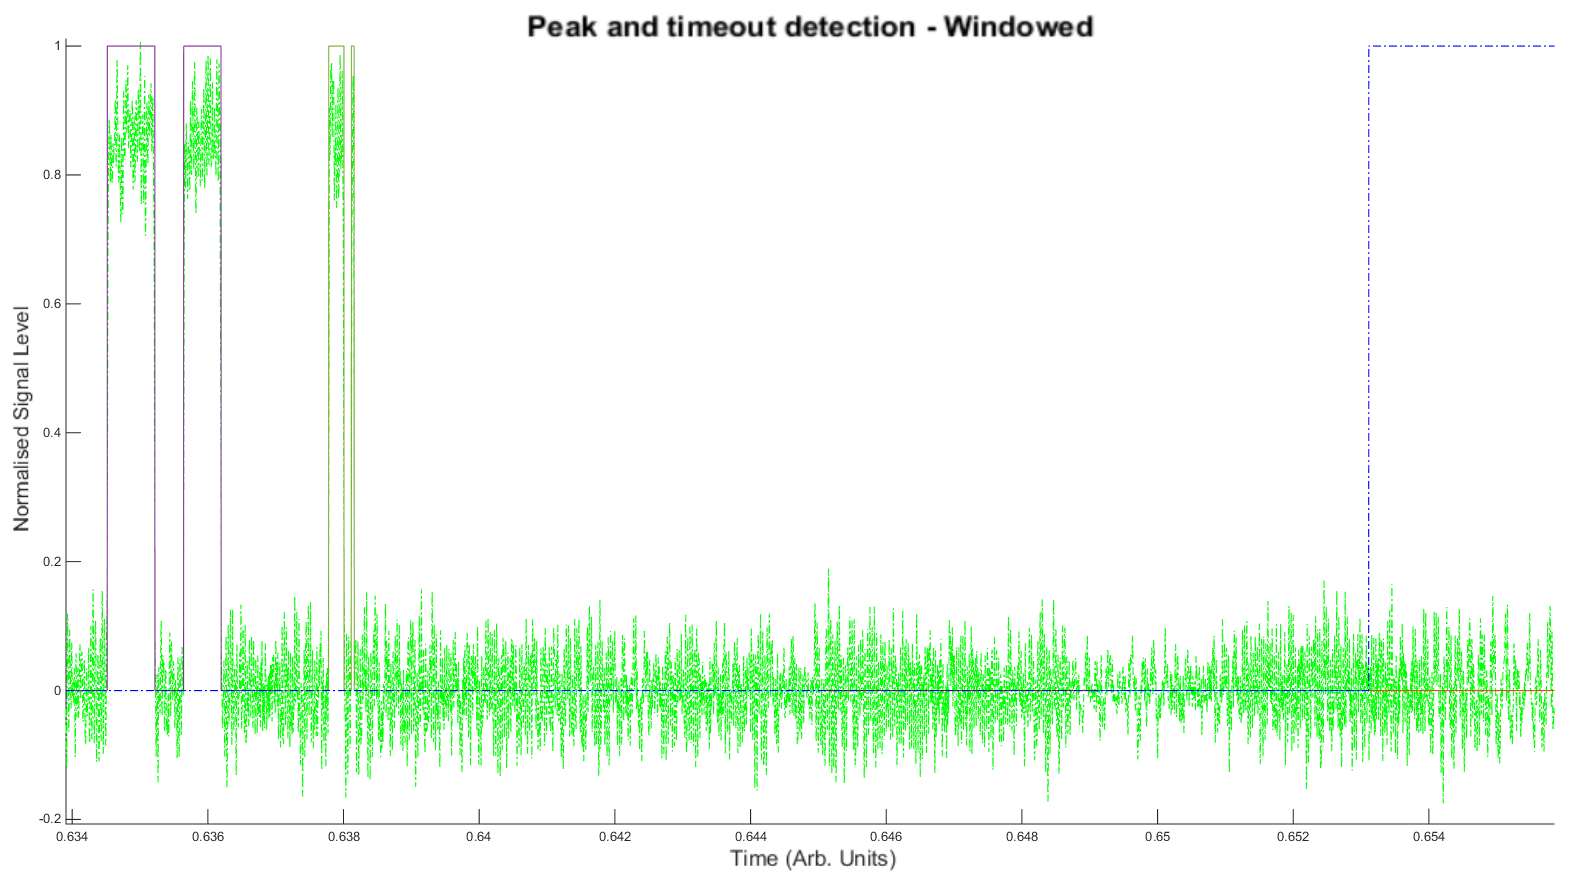
\includegraphics[width=\textwidth]{timeout_detection}
		\caption[MATLAB windowed peak detection on generated data]{MATLAB performing peak detection on windows of the green data set. The blue dashed line represents the output signal, once a set amount of time has passed}
		\label{fig::timeout_detection}
	\end{figure}
